\documentclass[11pt,psfig]{article}
\usepackage{epsfig}
\usepackage{times}
\usepackage{amssymb}
\usepackage{float}

\newcount\refno\refno=1
\def\ref{\the\refno \global\advance\refno by 1}
\def\ux{\underline{x}}
\def\uw{\underline{w}}
\def\bw{\underline{w}}
\def\ut{\underline{\theta}}
\def\umu{\underline{\mu}} 
\def\bmu{\underline{\mu}} 
\def\be{p_e^*}
\newcount\eqnumber\eqnumber=1
\def\eq{\the \eqnumber \global\advance\eqnumber by 1}
\def\eqs{\eq}
\def\eqn{\eqno(\eq)}

 \pagestyle{empty}
\def\baselinestretch{1.1}
\topmargin1in \headsep0.3in
\topmargin0in \oddsidemargin0in \textwidth6.5in \textheight8.5in
\begin{document}
\setlength{\parskip}{1.2ex plus0.3ex minus 0.3ex}


\thispagestyle{empty} \pagestyle{myheadings} \markright{G}



\title{CS 266 Homework 6}
\author{Zachary DeStefano, PhD Student, 15247592}
\date{Due Date: May 22}

\maketitle

\vfill\eject

\section*{Problem 6.13}

As a vertical line sweeps across, it will be making a trapezoid. \\
At a left endpoint, there are three trapezoids:\\
1. One already existing to the left of the new segment\\
2. One being made above existing segment to the right\\
3. One being made below existing segment to the right\\
\\
At a right endpoint, there are three trapezoids:\\
1. One already existing to the left above the old segment\\
2. One alright existing to the left below the old segment\\
3. One being made to the right of the old segment\\
\\
There are n segments that have left and right endpoints and at a left endpoint, there are 2 being made while at the right endpoint, there is one being made, thus for each segment, 3 trapezoids are made. With the very first endpoint though, 4 trapezoids are made because there is not one already existing to the left and it has to be made. Thus there are at most $3n+1$ trapezoids. 

\section*{Problem 6.15}

 Although we have started with the point location problem on the surface
of the earth, we have only treated planar point location. But the earth is
a globe. How would you define a spherical subdivision—a subdivision
of the surface of a sphere? Give a point location structure for such a
subdivision.\\
\\
Divide the sphere into cross-sections by x-coordinate. The top and bottom ones would be degenerate ones. You then divide up the cross-sections. \\
\\
Identically, each point on the surface of the sphere can be described by two angles $(\theta,\phi)$. You can take these coordinates for each point and put them into a 2-D space and then do the point location map. Vertical segments will correspond to the cross sections described above. 

\newpage

\section*{Problem 12.4}

If we have a set of segments such that each line will split at least one other segment, then the auto-partitions will have more nodes in the trees than the least possible partition. \\
\\
Here is an example of 3 line segments to partition:
\begin{figure}[H]
\centering
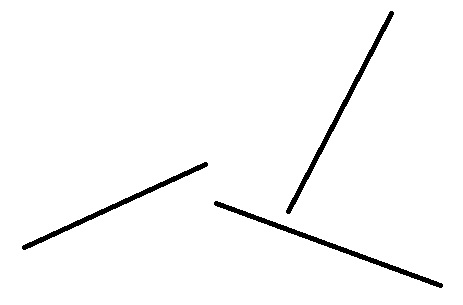
\includegraphics[height=3in]{hw6prob3diagram1.jpg}
\caption{Set of Line Segments to Partition}
\end{figure}

Here is a binary space partition that uses only 3 segments:
\begin{figure}[H]
\centering
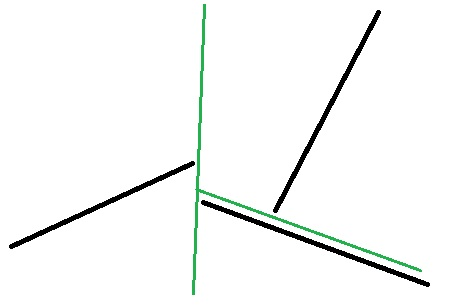
\includegraphics[height=3in]{hw6prob3diagram2.jpg}
\caption{Set of Line Segments Partitioned using the green lines}
\end{figure}

Each auto-partition will split up another line, thus at least 4 nodes are needed for an auto-partition, as can be seen with this example one
\begin{figure}[H]
\centering
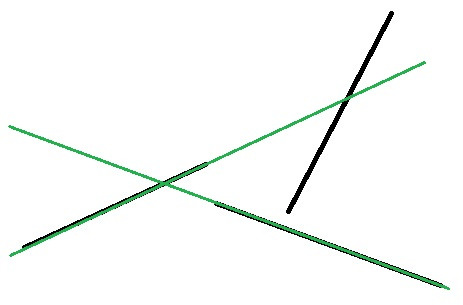
\includegraphics[height=3in]{hw6prob3diagram3.jpg}
\caption{Set of Line Segments with auto-partitioning lines in green}
\end{figure}

\section*{Problem 12.10}

%\begin{figure}[H]
%\centering
%\includegraphics[height=4in]{prob1plot.jpg}
%\caption{Probability of Class Labels with decision boundaries marked}
%\end{figure}


\end{document}








